\section{DATASET}

\subsection{Source and Collection}
The dataset is derived from tweet-style text collected using \texttt{snscrape}. Data collection was performed by issuing queries per emoji and retaining text samples that contain the queried emoji. English filtering is performed using \texttt{pycld3}, inspired by the WiLI language identification benchmark \cite{thoma2018wili}. Because scraped social media text is noisy, some non-English samples and duplicates may remain.

\subsection{Cleaning and Normalization}
The preprocessing notebook (\texttt{data-preprocess.ipynb}) applies a simple cleaning function that:
\begin{itemize}
    \item Removes URLs, mentions, hashtags, and emojis.
    \item Lowercases and collapses repeated whitespace.
\end{itemize}

\subsection{Data Samples}
Figure~\ref{fig:data-samples} shows a few data samples after cleaning.

\begin{figure}[H]
    \centering
    \includegraphics[width=0.7\linewidth]{images/data_samples.png}
    \caption{Example data samples after cleaning.}
    \label{fig:data-samples}
\end{figure}

\subsection{Train/Test Split Statistics}
The final dataset is stored as two CSV files (\texttt{data/train\_data.csv}, \texttt{data/test\_data.csv}). Table~\ref{tab:dataset-stats} summarizes the split.

\begin{table}[H]
    \centering
    \caption{Dataset statistics.}
    \label{tab:dataset-stats}
    \begin{tabular}{lrrr}
        \toprule
        Split & Samples & \#Classes & Class count range \\
        \midrule
        Train & 751{,}885 & 43 & 16{,}718--17{,}846 \\
        Test  & 83{,}543  & 43 & 1{,}858--1{,}983 \\
        \bottomrule
    \end{tabular}
\end{table}

\section{MODELS}

\subsection{TF--IDF Baseline Models}

As strong non-neural baselines, we employ linear classifiers trained on sparse TF--IDF representations. Given a document corpus, each text is mapped to a high-dimensional feature vector using a union of:
\begin{itemize}
    \item word $n$-grams (e.g., $n \in \{1,2\}$), which capture lexical content and short phrase-level semantics;
    \item character $n$-grams (e.g., $n \in \{3,4,5\}$), which are effective for modeling morphological patterns, misspellings, and informal language.
\end{itemize}

For each $n$-gram feature $t$ in document $d$, TF--IDF weighting is computed as
\[
\text{tfidf}(t,d) = \text{tf}(t,d) \cdot \log \frac{N}{\text{df}(t)},
\]
where $\text{tf}(t,d)$ denotes term frequency, $\text{df}(t)$ is document frequency, and $N$ is the total number of documents. This weighting downscales frequent but uninformative tokens while emphasizing discriminative ones. The resulting sparse vectors are used to train the following classifiers:

\paragraph{Linear Support Vector Machine.}
The linear SVM learns a maximum-margin hyperplane separating classes in the feature space. By maximizing the margin between decision boundaries and minimizing hinge loss, it tends to generalize well in high-dimensional sparse settings typical of text data.

\begin{figure}[H]
    \centering
    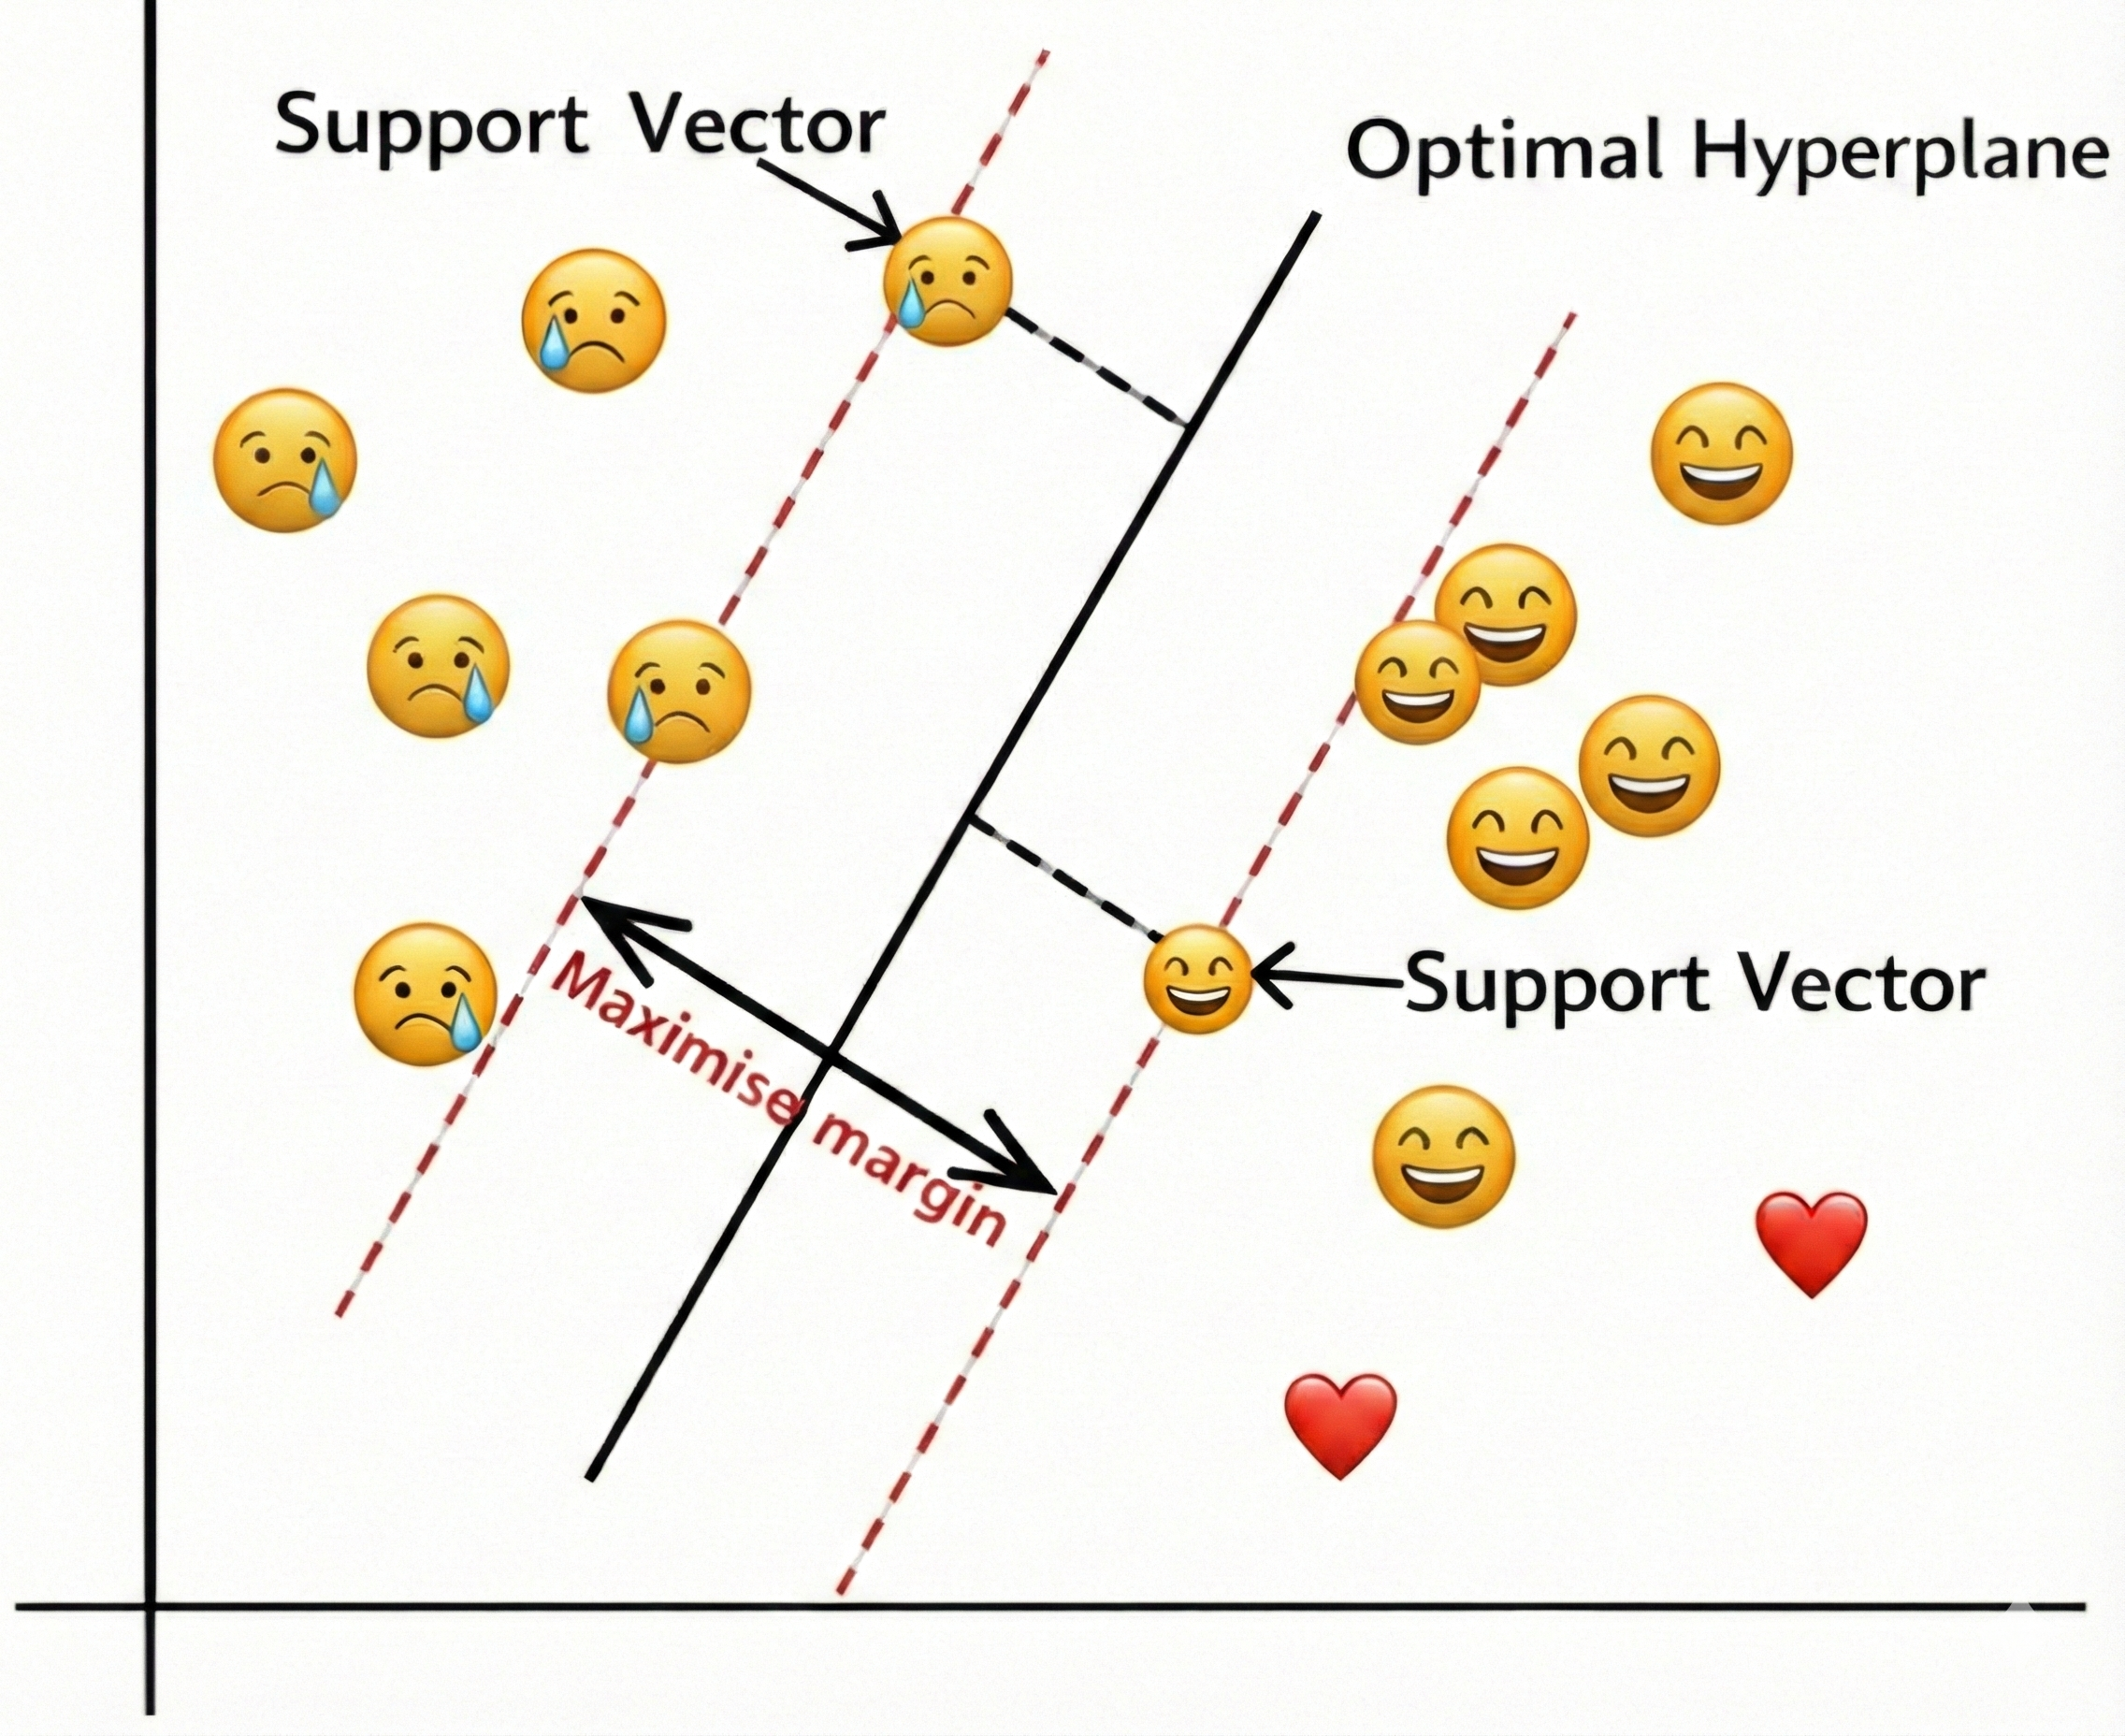
\includegraphics[width=0.4\linewidth]{images/svm.png}
    \caption{Linear Support Vector Machine.}
    \label{fig:svm}
\end{figure}

\paragraph{Logistic Regression.}
Let each document be represented by a TF--IDF feature vector $\mathbf{x}\in\mathbb{R}^d$ and let there be $C$ classes. Logistic regression defines linear class scores (logits)
\[
\mathbf{z} = \mathbf{W}\mathbf{x} + \mathbf{b},
\]
where $\mathbf{W}\in\mathbb{R}^{C\times d}$ and $\mathbf{b}\in\mathbb{R}^{C}$. The conditional probability of class $c$ is computed via the softmax function:
\[
p(y=c\mid \mathbf{x})=\frac{\exp(z_c)}{\sum_{j=1}^{C}\exp(z_j)}.
\]
Training typically minimizes the negative log-likelihood (cross-entropy) with $\ell_2$ regularization:
\[
\mathcal{L}(\mathbf{W},\mathbf{b})
= -\sum_{i=1}^{N}\log p\!\left(y_i \mid \mathbf{x}_i\right)
\;+\;\lambda \|\mathbf{W}\|_2^2.
\]

\paragraph{Multinomial Naive Bayes.}
Multinomial Naive Bayes is a generative probabilistic model over discrete features (typically word or $n$-gram counts). Let $\mathbf{x}=(x_1,\dots,x_V)$ be the count vector over a vocabulary of size $V$. Under the conditional independence assumption,
\[
p(\mathbf{x}\mid y=c)=\prod_{j=1}^{V} p(w_j\mid c)^{x_j}.
\]
With class prior $p(y=c)$, Bayes' rule yields the posterior (up to normalization):
\[
p(y=c\mid \mathbf{x}) \propto p(y=c)\prod_{j=1}^{V} p(w_j\mid c)^{x_j}.
\]
In practice, prediction is performed in log-space:
\[
\hat{y}=\arg\max_{c}\left[\log p(y=c)+\sum_{j=1}^{V} x_j \log p(w_j\mid c)\right].
\]
The parameters are estimated from training counts using Laplace smoothing ($\alpha>0$):
\[
\hat{p}(w_j\mid c)=\frac{N_{jc}+\alpha}{\sum_{t=1}^{V}N_{tc}+\alpha V},
\qquad
\hat{p}(y=c)=\frac{N_c}{N},
\]
where $N_{jc}$ denotes the total count of token $w_j$ in class $c$, $N_c$ is the number of documents in class $c$, and $N$ is the total number of documents.

\subsection{FastText-Style Subword Model}

We adopt a FastText-style linear text classifier \cite{joulin2017bag} that combines the efficiency of bag-of-features models with the robustness of subword representations. The key idea is to represent a document by an aggregated embedding of its observed tokens, where each token embedding is augmented with character-level $n$-gram features. This design greatly reduces the impact of data sparsity and allows the model to generalize to rare spellings and out-of-vocabulary (OOV) words that are common in informal social media text.

\paragraph{Subword decomposition and hashing.}
Given a token $w$, we first generate its set of character $n$-grams $G(w)$, typically for $n \in [n_{\min}, n_{\max}]$ (e.g., 3--6). Each $n$-gram $g \in G(w)$ is mapped to an integer index using a hashing function
\[
h(g) \in \{1,2,\dots,B\},
\]
where $B$ is the number of hashing buckets. Hashing provides a fixed-size parameterization independent of the vocabulary size, keeping memory usage bounded while still allowing the model to share statistical strength across morphologically related strings. Collisions may occur, but in practice a sufficiently large $B$ yields good performance with modest memory.

\paragraph{Token representation.}
The embedding of a token is computed by combining a learned word-level vector with the vectors of its subword $n$-grams. Let $\mathbf{u}_w \in \mathbb{R}^d$ denote the word embedding for token $w$ (when available) and let $\mathbf{v}_{h(g)} \in \mathbb{R}^d$ denote the embedding of the bucket to which $n$-gram $g$ is hashed. The token representation is
\[
\mathbf{x}(w) \;=\; \mathbf{u}_w \;+\; \sum_{g \in G(w)} \mathbf{v}_{h(g)}.
\]
This construction allows the model to form a meaningful vector even when $w$ is rare or unseen: as long as its character $n$-grams have been observed during training, the subword sum provides a robust estimate of its semantics.

\paragraph{Document representation.}
For a document $D$ consisting of tokens $(w_1,\dots,w_T)$, we compute a single document vector by averaging token representations:
\[
\mathbf{z}(D) \;=\; \frac{1}{T}\sum_{t=1}^{T}\mathbf{x}(w_t).
\]
Averaging yields an order-invariant (bag-of-embeddings) representation that is computationally lightweight: inference and training scale linearly with the number of tokens and the number of extracted subword $n$-grams.

\paragraph{Linear classifier and training objective.}
The document embedding is fed into a linear classification layer with parameters $(\mathbf{W},\mathbf{b})$:
\[
\mathbf{s}(D) = \mathbf{W}\mathbf{z}(D) + \mathbf{b},
\]
and class probabilities are produced via the softmax function $p(y \mid D)=\mathrm{softmax}(\mathbf{s}(D))$. The model is trained end-to-end by minimizing the cross-entropy loss over the training set:
\[
\mathcal{L} \;=\; -\sum_{(D,y)} \log p(y \mid D).
\]

Although this model discards word order, the inclusion of character $n$-grams injects morphological and orthographic information, improving generalization in noisy settings (misspellings, elongations, slang, and code-mixing). Consequently, FastText-style subword models often outperform purely count-based bag-of-words baselines under low-resource conditions while remaining significantly faster and simpler than deep sequence models \cite{joulin2017bag}.


\subsection{TextCNN}
\label{subsec:textcnn}

TextCNN \cite{kim2014cnn} applies convolutions over word embeddings to extract local, position-invariant $n$-gram features for classification. Given an input sentence (or post) tokenized into a sequence
$\mathbf{w} = (w_1, w_2, \dots, w_L)$ of length $L$, each token $w_i$ is mapped to a dense embedding
$\mathbf{x}_i \in \mathbb{R}^{d}$ via an embedding lookup table $\mathbf{E}\in\mathbb{R}^{|\mathcal{V}|\times d}$.
Stacking embeddings yields the sentence matrix:
\begin{equation}
\mathbf{X} =
\begin{bmatrix}
\mathbf{x}_1^\top\\
\mathbf{x}_2^\top\\
\vdots\\
\mathbf{x}_L^\top
\end{bmatrix}
\in \mathbb{R}^{L\times d}.
\end{equation}
In practice, sequences are padded/truncated to a maximum length (e.g., per-batch maximum or a global $L_{\max}$) to enable batched computation.

\paragraph{Convolution over embeddings.}
To capture patterns of different $n$-gram lengths, TextCNN uses multiple convolutional filter widths $k \in \mathcal{K}$ (e.g., $\{3,4,5\}$).
For a given width $k$, let $\mathbf{W}^{(k,j)}\in\mathbb{R}^{k\times d}$ and $b^{(k,j)}\in\mathbb{R}$ denote the parameters
of the $j$-th filter (out of $m_k$ filters) for that width. The convolution is applied to each contiguous window
$\mathbf{X}_{i:i+k-1}\in\mathbb{R}^{k\times d}$:
\begin{equation}
c^{(k,j)}_i = \phi\!\left( \langle \mathbf{W}^{(k,j)}, \mathbf{X}_{i:i+k-1} \rangle + b^{(k,j)} \right),
\quad i=1,\dots,L-k+1,
\end{equation}
where $\langle \cdot,\cdot\rangle$ denotes the Frobenius inner product and $\phi(\cdot)$ is a nonlinearity (typically ReLU).
This produces a feature map $\mathbf{c}^{(k,j)} \in \mathbb{R}^{L-k+1}$ for each filter.

\paragraph{Global max-over-time pooling.}
To convert variable-length feature maps into fixed-dimensional features, TextCNN performs max-over-time pooling:
\begin{equation}
\hat{c}^{(k,j)} = \max_{1\le i\le L-k+1} c^{(k,j)}_i .
\end{equation}
Intuitively, each filter learns to detect a particular local pattern, and max pooling retains the strongest activation
anywhere in the sequence, making the representation largely insensitive to the pattern’s position.

\paragraph{Classification head.}
All pooled scalars are concatenated into a single vector:
\begin{equation}
\mathbf{h} =
\big[ \hat{c}^{(k,1)}, \dots, \hat{c}^{(k,m_k)} \big]_{k\in\mathcal{K}}
\in \mathbb{R}^{\sum_{k\in\mathcal{K}} m_k}.
\end{equation}
We apply dropout to $\mathbf{h}$ for regularization and use a linear layer to predict logits over classes:
\begin{equation}
\mathbf{z} = \mathbf{W}_o \,\mathrm{Dropout}(\mathbf{h}) + \mathbf{b}_o,
\qquad
p(y=c \mid \mathbf{w}) = \mathrm{softmax}(\mathbf{z})_c .
\end{equation}
The model is trained end-to-end with cross-entropy loss.

TextCNN is computationally efficient (highly parallelizable) and effective at capturing local syntactic/semantic cues
useful for text classification. However, its receptive field is limited to the largest filter width and it does not
explicitly model long-range dependencies beyond what can be inferred from local cues and pooling.

\begin{figure}[t]
\centering
\includegraphics[width=\linewidth]{images/textcnn.png}
\caption{TextCNN architecture with multiple filter widths and global max-over-time pooling.}
\label{fig:textcnn}
\end{figure}


\subsection{Bidirectional RNN with Attention}

Recurrent neural networks (RNNs) explicitly model sequential structure by processing tokens in order. This inductive bias is useful for short, informal social media text where meaning can depend on word order (e.g., negation, intensifiers, and short multiword expressions). We consider two gated RNN variants---LSTM and GRU---and use a bidirectional encoder so that each token representation incorporates both left and right context.

\paragraph{Input representation.}
Given a tokenized text $\mathbf{w} = (w_1,w_2,\dots,w_L)$ of length $L$, each token $w_i$ is mapped to an embedding $\mathbf{x}_i \in \mathbb{R}^{d}$ using a learned lookup table $\mathbf{E}\in\mathbb{R}^{|\mathcal{V}|\times d}$. To enable batched training, sequences are padded/truncated to a maximum length $L_{\max}$, and we maintain a binary padding mask to distinguish real tokens from padded positions.

\begin{figure}[t]
\centering
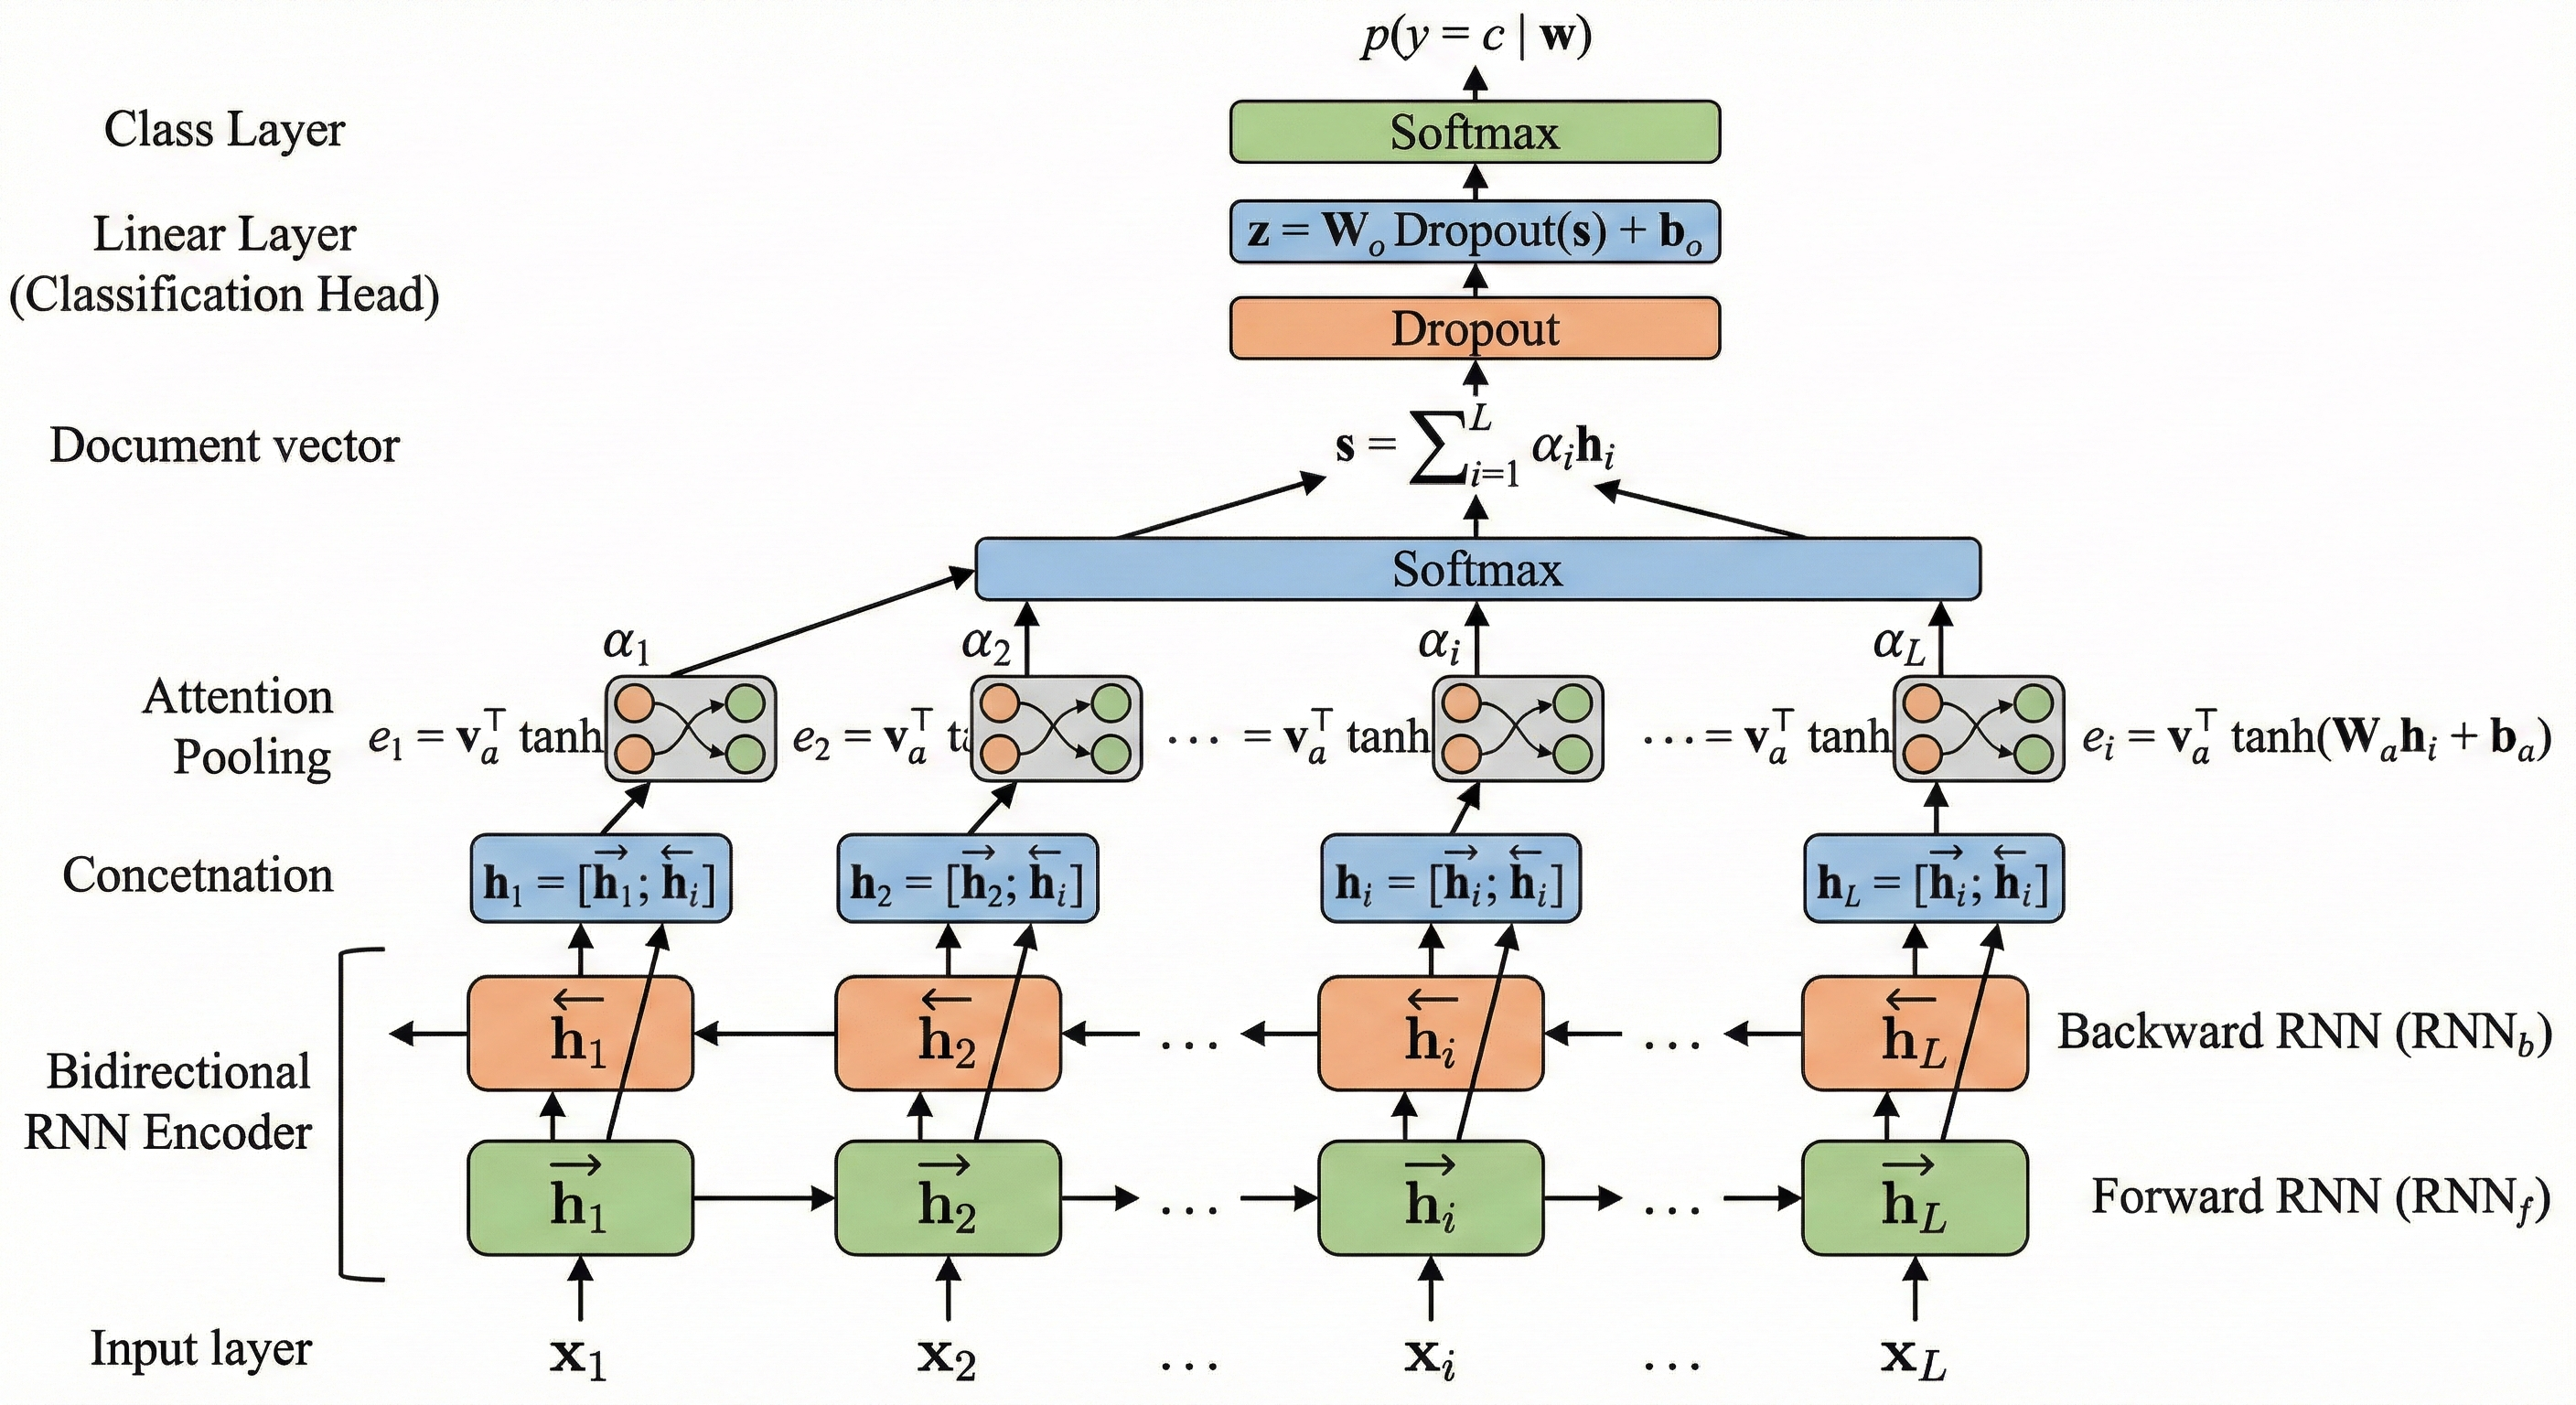
\includegraphics[width=\linewidth]{images/rnn.png}
\caption{Bidirectional RNN with additive attention pooling for text classification.}
\label{fig:birnn_attention}
\end{figure}

\paragraph{Bidirectional recurrent encoder.}
A forward RNN reads the sequence from left to right, while a backward RNN reads it from right to left:
\begin{align}
\overrightarrow{\mathbf{h}}_i &= \mathrm{RNN}_f(\mathbf{x}_i, \overrightarrow{\mathbf{h}}_{i-1}),\\
\overleftarrow{\mathbf{h}}_i &= \mathrm{RNN}_b(\mathbf{x}_i, \overleftarrow{\mathbf{h}}_{i+1}).
\end{align}
The contextual token representation is the concatenation of both directions,
\begin{equation}
\mathbf{h}_i = \left[\overrightarrow{\mathbf{h}}_i;\overleftarrow{\mathbf{h}}_i\right] \in \mathbb{R}^{2h},
\end{equation}
where $h$ is the hidden size per direction. Gated cells (LSTM/GRU) mitigate vanishing gradients and allow the model to retain salient information over longer spans compared to a vanilla RNN.

\paragraph{Additive attention pooling.}
To aggregate token-level information into a single fixed-dimensional document vector, we apply an additive attention mechanism \cite{bahdanau2015neural}. Each hidden state is scored by a small feed-forward network:
\begin{align}
e_i &= \mathbf{v}_a^\top \tanh(\mathbf{W}_a \mathbf{h}_i + \mathbf{b}_a),\\
\alpha_i &= \frac{\exp(e_i)}{\sum_{j=1}^{L}\exp(e_j)},
\end{align}
where $\mathbf{W}_a \in \mathbb{R}^{r\times 2h}$, $\mathbf{b}_a\in\mathbb{R}^{r}$, and $\mathbf{v}_a \in \mathbb{R}^{r}$ are learned parameters. In batched training, the padding mask is used so that padded positions do not receive probability mass. The resulting document representation is a weighted sum of hidden states:
\begin{equation}
\mathbf{s} = \sum_{i=1}^{L} \alpha_i \mathbf{h}_i \in \mathbb{R}^{2h}.
\end{equation}
Intuitively, attention learns to assign higher weights to tokens that are more predictive of the target emoji (e.g., sentiment-bearing words, named entities, or topic keywords), and the weights can be inspected to provide a degree of interpretability.

\paragraph{Classification head and training objective.}
The attended vector $\mathbf{s}$ is regularized with dropout and passed to a linear layer to obtain class logits:
\begin{equation}
\mathbf{z} = \mathbf{W}_o\,\mathrm{Dropout}(\mathbf{s}) + \mathbf{b}_o,
\qquad
p(y=c\mid \mathbf{w}) = \mathrm{softmax}(\mathbf{z})_c.
\end{equation}
The model is trained end-to-end by minimizing cross-entropy loss. In practice, gradient clipping is commonly used to stabilize optimization for recurrent networks.

Compared to uniform average/max pooling, attention provides a task-adaptive summary of the sequence. Relative to convolutional models such as TextCNN, bidirectional RNNs can capture dependencies spanning many tokens, but they are less parallelizable and typically slower due to the sequential nature of recurrent computation.

\subsection{Transformer-Based Model: DistilBERT Fine-Tuning}

We fine-tune DistilBERT \cite{sanh2019distilbert}, a compact Transformer encoder distilled from BERT \cite{devlin2019bert}, for multi-class emoji prediction. Transformer encoders model contextual meaning through stacked self-attention blocks \cite{vaswani2017attention}, allowing each token to attend to all others and capture both local and long-range interactions.

\paragraph{Subword tokenization and inputs.}
Given an input text, a WordPiece-style tokenizer \cite{devlin2019bert} converts it into a sequence of subword tokens and inserts special tokens to form
\[
(\texttt{[CLS]}, t_1, \dots, t_T, \texttt{[SEP]}),
\]
where $T$ varies per example. Each token is mapped to an integer ID, and sequences are padded/truncated to a fixed maximum length $L_{\max}$ for batching. We also create an attention mask $\mathbf{m}\in\{0,1\}^{L_{\max}}$ indicating which positions correspond to real tokens (1) versus padding (0); the mask prevents padded positions from influencing attention scores.

\paragraph{Embedding layer.}
Let $d$ be the model hidden size. The input IDs are mapped to token embeddings and combined with learned positional embeddings:
\begin{equation}
\mathbf{x}_i = \mathbf{e}_{\text{tok}}(t_i) + \mathbf{e}_{\text{pos}}(i) \in \mathbb{R}^{d},
\qquad i=1,\dots,L_{\max}.
\end{equation}
DistilBERT uses a single-sequence encoder and therefore omits segment (token-type) embeddings used in some BERT variants \cite{sanh2019distilbert}.

\paragraph{Multi-head self-attention.}
Given the hidden states from layer $\ell-1$, stacked into a matrix $\mathbf{H}^{(\ell-1)}\in\mathbb{R}^{L_{\max}\times d}$, each attention head computes query, key, and value projections:
\begin{equation}
\mathbf{Q}=\mathbf{H}^{(\ell-1)}\mathbf{W}^{Q},\quad
\mathbf{K}=\mathbf{H}^{(\ell-1)}\mathbf{W}^{K},\quad
\mathbf{V}=\mathbf{H}^{(\ell-1)}\mathbf{W}^{V}.
\end{equation}
Self-attention produces contextualized representations by weighting values based on similarity between queries and keys:
\begin{equation}
\mathrm{Attn}(\mathbf{Q},\mathbf{K},\mathbf{V}) =
\mathrm{softmax}\!\left(\frac{\mathbf{Q}\mathbf{K}^{\top}}{\sqrt{d_k}} + \mathbf{M}\right)\mathbf{V},
\end{equation}
where $d_k$ is the per-head key dimension and $\mathbf{M}$ is a masking matrix derived from $\mathbf{m}$ that assigns large negative values to padded positions so they receive near-zero attention probability. Multiple heads are computed in parallel and concatenated, followed by an output projection (omitted for brevity) \cite{vaswani2017attention}.

\begin{figure}[t]
\centering
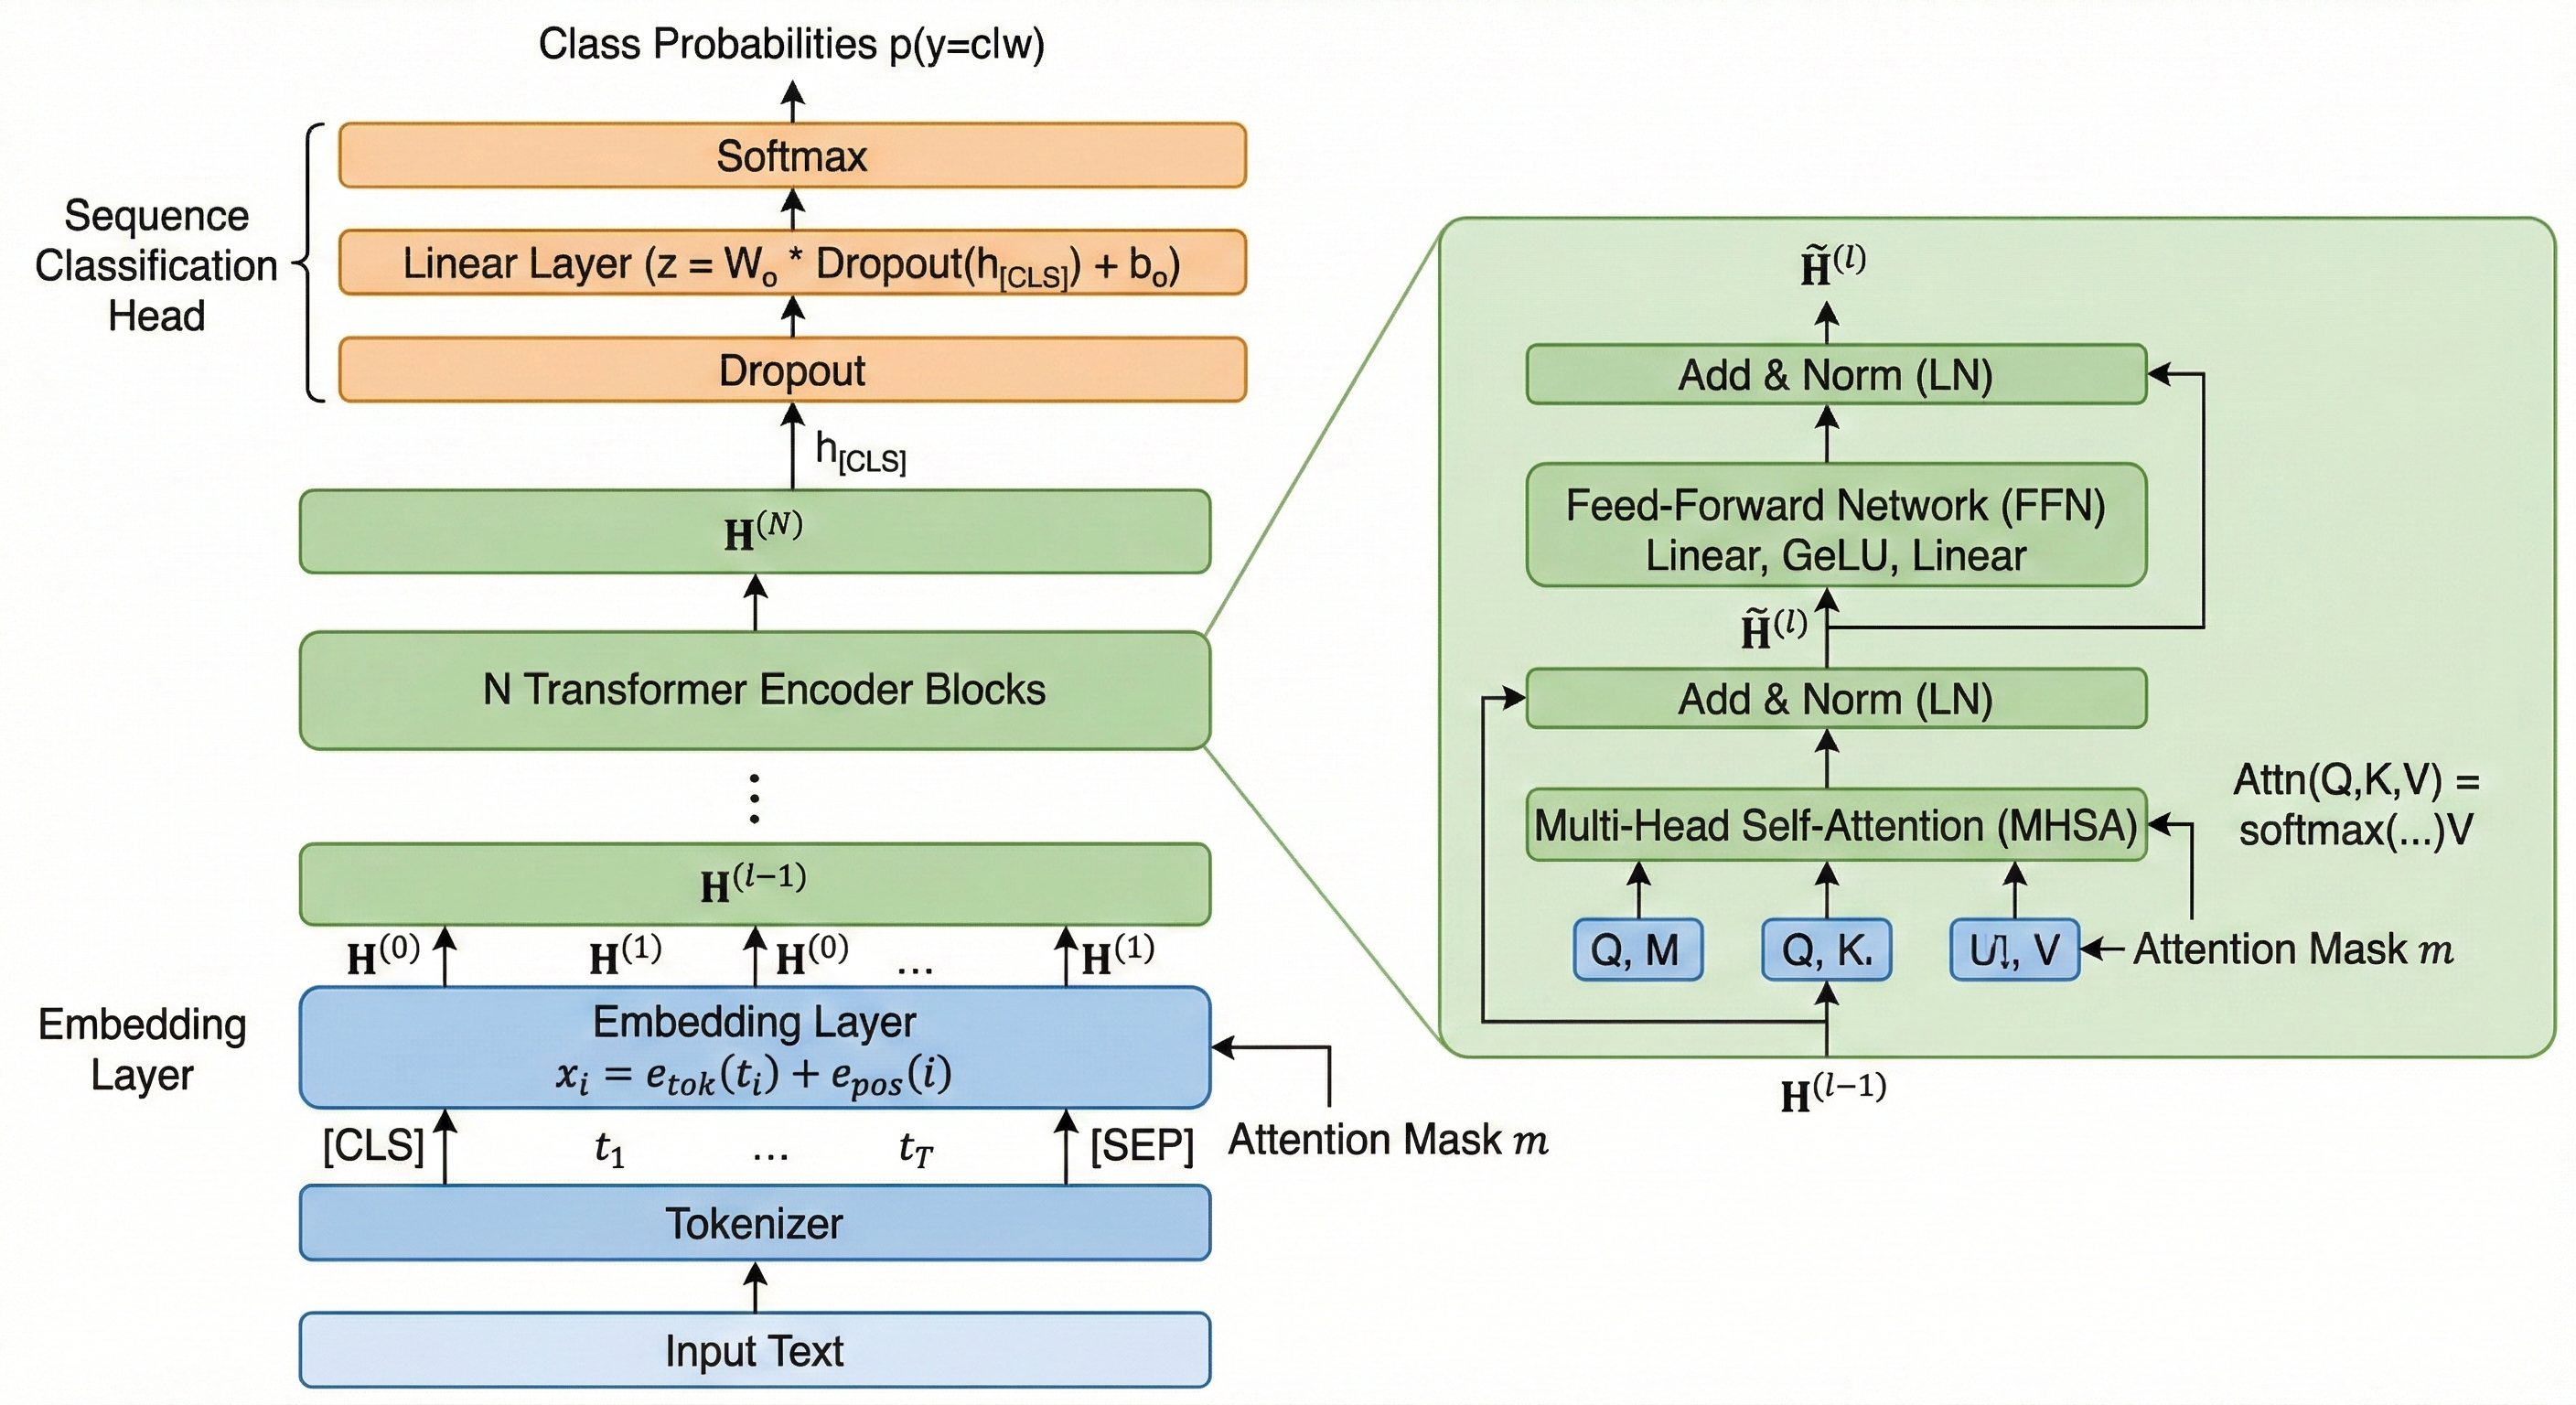
\includegraphics[width=\linewidth]{images/bert.png}
\caption{DistilBERT architecture overview.}
\label{fig:bert}    
\end{figure}

\paragraph{Transformer encoder block.}
Each layer applies self-attention and a position-wise feed-forward network with residual connections and layer normalization:
\begin{align}
\tilde{\mathbf{H}}^{(\ell)} &= \mathrm{LN}\!\left(\mathbf{H}^{(\ell-1)} + \mathrm{Dropout}(\mathrm{MHSA}(\mathbf{H}^{(\ell-1)}))\right),\\
\mathbf{H}^{(\ell)} &= \mathrm{LN}\!\left(\tilde{\mathbf{H}}^{(\ell)} + \mathrm{Dropout}(\mathrm{FFN}(\tilde{\mathbf{H}}^{(\ell)}))\right),
\end{align}
where $\mathrm{FFN}(\mathbf{h})=\mathbf{W}_2\,\sigma(\mathbf{W}_1\mathbf{h}+\mathbf{b}_1)+\mathbf{b}_2$ is applied independently to each position. Stacking $N$ such layers yields the final contextual sequence representation $\mathbf{H}^{(N)}$.

\paragraph{Sequence classification head and objective.}
For classification, we use the final hidden state corresponding to the \texttt{[CLS]} token as a pooled sequence representation, $\mathbf{h}_{\texttt{[CLS]}}\in\mathbb{R}^{d}$. A linear classifier maps it to logits over $C$ emoji classes:
\begin{equation}
\mathbf{z}=\mathbf{W}_o\,\mathrm{Dropout}(\mathbf{h}_{\texttt{[CLS]}})+\mathbf{b}_o,
\qquad
p(y=c\mid \mathbf{w})=\mathrm{softmax}(\mathbf{z})_c.
\end{equation}
All parameters are fine-tuned end-to-end by minimizing cross-entropy loss. In our implementation, we use AdamW optimization with a linear warmup/decay learning-rate schedule, which is standard for Transformer fine-tuning \cite{devlin2019bert}.

Compared to CNN/RNN architectures trained from scratch, DistilBERT benefits from large-scale pretraining and can leverage richer syntactic/semantic features. The main trade-off is higher computational cost and memory usage, though DistilBERT remains significantly smaller and faster than full-sized BERT \cite{sanh2019distilbert}.
